% ESE3990 intermediate presentation (3-minute video).
% Build: latexmk -pdf -outdir=build main.tex
% Numbers and figures: python make_figures.py (see script.md).
\documentclass[aspectratio=169,11pt]{beamer}

\usepackage{booktabs}
\usepackage{tikz}
\usetikzlibrary{arrows.meta,positioning,calc}

% --- NUS corporate colours (nus.edu.sg/identity/guidelines/corporate-colours)
\definecolor{nusblue}{HTML}{003D7C}
\definecolor{nusorange}{HTML}{EF7C00}

% --- One colour per controller, on every slide and figure (make_figures.py
%     uses the same hex values). RuleSailor is also dashed in graphs.
\definecolor{colPPO}{HTML}{5FAE5F}
\definecolor{colSAC}{HTML}{1F66CC}
\definecolor{colMPC}{HTML}{C71585}
\definecolor{colRule}{HTML}{6B6B6B}
\newcommand{\PPO}{\textcolor{colPPO}{PPO}}
\newcommand{\SAC}{\textcolor{colSAC}{SAC}}
\newcommand{\MPC}{\textcolor{colMPC}{MPC}}
\newcommand{\CEM}{\textcolor{colMPC}{CEM-MPC}}
\newcommand{\Rule}{\textcolor{colRule}{RuleSailor}}
% A block titled in its controller's colour.
\newenvironment{algblock}[3]{%
  \setbeamercolor{block title}{fg=white,bg=#2}%
  \setbeamercolor{block body}{bg=#2!8}%
  \begin{block}{#1 \hfill\normalfont\scriptsize #3}}{\end{block}}

% --- Course drawings in world metres (x east, y north), as the web frontend
%     draws them: a circle of the course half-width with the gate bar between
%     the two posts Rust's route builder returns.
\definecolor{gatecol}{HTML}{B22222}
\definecolor{hullline}{HTML}{2B3A45}
\definecolor{sailred}{HTML}{D64D3F}
\newcommand{\gate}[3]{%
  \draw[gatecol,line width=0.5pt] #1 circle (5);
  \draw[gatecol,line width=1.4pt] #2 -- #3;}
\newcommand{\wind}[2]{% top of the arrow, length (m)
  \draw[-{Stealth[length=1.6mm]},line width=1.2pt,black!60] #1 -- ++(0,-#2)
    node[below,font=\scriptsize,black!60] {wind};}
\tikzset{
  % ILCA hull 4.23 x 1.37 m (web HULL_OUTLINE), mast 1.2 m forward, 2.72 m
  % boom eased 30 deg to starboard; pic frame: x forward, y port, metres.
  boat/.pic={
    \filldraw[fill=white,draw=hullline,line width=0.4pt,line join=round]
      (2.115,0) -- (1.777,0.247) -- (1.058,0.521) -- (0.212,0.658) -- (-0.635,0.685)
      -- (-1.481,0.617) -- (-2.115,0.493) -- (-2.115,-0.493) -- (-1.481,-0.617)
      -- (-0.635,-0.685) -- (0.212,-0.658) -- (1.058,-0.521) -- (1.777,-0.247) -- cycle;
    \fill[sailred,opacity=0.35] (1.2,0) .. controls (0.3,-1.25) .. (-1.156,-1.36) -- cycle;
    \draw[sailred,line width=0.6pt] (1.2,0) -- (-1.156,-1.36);
    \fill[hullline] (1.2,0) circle (0.13);
  },
}

\setbeamercolor{structure}{fg=nusblue}
\setbeamercolor{title}{fg=white,bg=nusblue}
\setbeamercolor{frametitle}{fg=white,bg=nusblue}
\setbeamercolor{item}{fg=nusorange}
\setbeamercolor{alerted text}{fg=nusorange}
\setbeamercolor{block title}{fg=white,bg=nusblue}
\setbeamercolor{block body}{bg=nusblue!6}
\setbeamercolor{footline}{fg=nusblue!70}
\setbeamercolor{titlerule}{bg=nusorange}
\setbeamertemplate{navigation symbols}{}
\setbeamertemplate{blocks}[rounded]
\setbeamertemplate{frametitle}{%
  \nointerlineskip
  \begin{beamercolorbox}[wd=\paperwidth,ht=2.6ex,dp=1.3ex,leftskip=1.2em]{frametitle}%
    \usebeamerfont{frametitle}\insertframetitle
  \end{beamercolorbox}%
  \nointerlineskip
  \begin{beamercolorbox}[wd=\paperwidth,ht=2pt,dp=0pt]{titlerule}\end{beamercolorbox}%
}
\setbeamertemplate{footline}{%
  \usebeamercolor[fg]{footline}\scriptsize
  \hspace{1.2em}Shimin Chen \textperiodcentered{} ESE3990\hfill
  \insertframenumber\,/\,\inserttotalframenumber\hspace{1.2em}\vspace{0.8ex}%
}

% Generated by make_figures.py from runs/ese3990; do not edit.
\newcommand{\rPPOtest}{0/150}
\newcommand{\rSACtest}{117/150}
\newcommand{\rMPCtest}{150/150}
\newcommand{\rRULEtest}{50/50}
\newcommand{\rPPOshift}{0/60}
\newcommand{\rSACshift}{22/60}
\newcommand{\rMPCshift}{60/60}
\newcommand{\rRULEshift}{20/20}
\newcommand{\uPPOtest}{0/150}
\newcommand{\uPPOBCtest}{0/150}
\newcommand{\uBCtest}{0/150}
\newcommand{\uSACtest}{0/150}
\newcommand{\uSACDtest}{5/150}
\newcommand{\uMPCtest}{96/96}
\newcommand{\uMPCshift}{0/0}
\newcommand{\uRULEtest}{38/50}
\newcommand{\uRULEshift}{2/20}
\newcommand{\uMPCvalShort}{0/60}
\newcommand{\uMPCvalLong}{60/60}
\newcommand{\uMPCpLong}{193}
\newcommand{\uMPCpShort}{48}
\newcommand{\uMPCpartial}{partial: 96/210 episodes}

\graphicspath{{figs/}}

\title{Learning versus Planning for Sailboat Control}
\subtitle{\textbf{PPO}, \textbf{SAC} and true-model \textbf{MPC} in \textit{Sailgym}}
\author{Shimin Chen}
\institute{ESE3990 \textperiodcentered{} Intermediate presentation}
\date{13 November 2026}

\begin{document}

% ---------------------------------------------------------------- 0:00
\begin{frame}[plain]
  \titlepage
\end{frame}

% ---------------------------------------------------------------- after the live demo
\begin{frame}{The problem: you cannot sail straight at the wind}
  \begin{columns}[T]
    \begin{column}{0.44\textwidth}
      \centering
      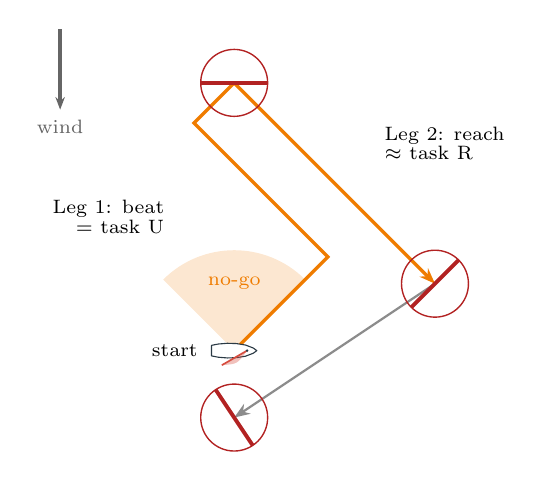
\begin{tikzpicture}[x=0.085cm,y=0.085cm,>={Stealth[length=2mm]}]
        % no-go zone at the start
        \fill[nusorange!18] (0,0) -- (45:15) arc[start angle=45,end angle=135,radius=15] -- cycle;
        \node[nusorange,font=\scriptsize] at (0,10) {no-go};
        \wind{(-26,48)}{12}
        % leg 1: beat (task U), drawn as two tacks; leg 2: reach (like task R)
        \draw[nusorange,very thick] (0,0) -- (14,14) -- (-6,34) -- (0,40);
        \draw[->,nusorange,very thick] (0,40) -- (30,10);
        \draw[->,black!45,thick] (30,10) -- (0,-10);
        % gates: posts from sailgym_core.route_waypoints (courses/triangle.json)
        \gate{(0,40)}{(5,40)}{(-5,40)}
        \gate{(30,10)}{(26.46,6.46)}{(33.54,13.54)}
        \gate{(0,-10)}{(-2.77,-5.84)}{(2.77,-14.16)}
        \pic[scale=1.6] at (0,0) {boat};
        \node[font=\scriptsize,anchor=east] at (-4,0) {start};
        \node[font=\scriptsize,align=right,anchor=east] at (-9,20) {Leg 1: beat\\[-1pt]\alert{= task U}};
        \node[font=\scriptsize,align=left,anchor=west] at (21,31) {Leg 2: reach\\[-1pt]\alert{$\approx$ task R}};
      \end{tikzpicture}\\[2pt]
      {\scriptsize Triangle course, as sailed in the web demo}
    \end{column}
    \begin{column}{0.54\textwidth}
      \begin{itemize}
        \item Controls are \alert{rates}: rudder and sheet, 20 times a second
        \item The physics decides heel, speed, capsize and whether the gate is passed
        \item Upwind needs a \alert{tack}: zig-zag through the no-go zone without stalling ``in irons''
      \end{itemize}
      \vspace{0.6em}
      \begin{block}{Question}
        How do on-policy learning, off-policy learning and planning with a known model trade off
        \alert{success}, \alert{experience} and \alert{computation}?
      \end{block}
    \end{column}
  \end{columns}
\end{frame}

% ---------------------------------------------------------------- 1:00
\begin{frame}{Method: one simulator, one contract for every controller}
  \centering
  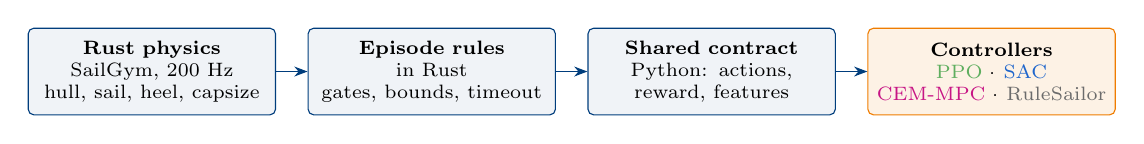
\begin{tikzpicture}[node distance=4mm,
      box/.style={draw=nusblue,fill=nusblue!6,rounded corners=2pt,align=center,
                  font=\scriptsize,text width=3.0cm,minimum height=1.1cm,inner sep=2pt}]
    \node[box] (phys) {\textbf{Rust physics}\\SailGym, 200 Hz\\hull, sail, heel, capsize};
    \node[box,right=of phys] (ep) {\textbf{Episode rules}\\in Rust\\gates, bounds, timeout};
    \node[box,right=of ep] (con) {\textbf{Shared contract}\\Python: actions,\\reward, features};
    \node[box,right=of con,draw=nusorange,fill=nusorange!10] (ctl) {\textbf{Controllers}\\\PPO{} \textperiodcentered{} \SAC\\\CEM{} \textperiodcentered{} \Rule};
    \foreach \a/\b in {phys/ep,ep/con,con/ctl} \draw[-{Stealth},nusblue] (\a) -- (\b);
  \end{tikzpicture}\\[1.2em]
  \begin{columns}[c]
    \begin{column}{0.50\textwidth}
      \centering
      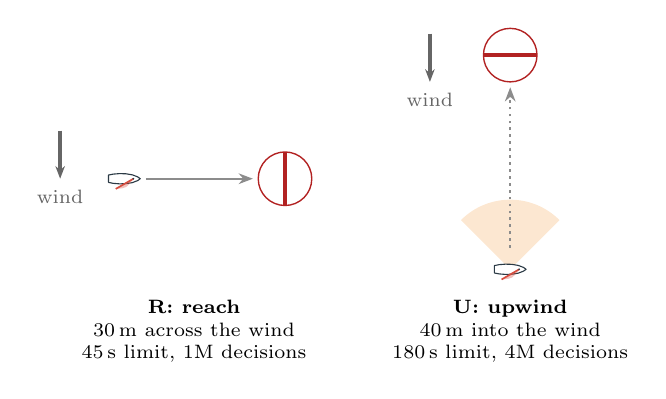
\begin{tikzpicture}[x=0.068cm,y=0.068cm,>={Stealth[length=1.8mm]}]
        % R: first leg of courses/reach.json, drawn at mid-height of U
        \begin{scope}[yshift=1.15cm]
          \wind{(-12,9)}{9}
          \draw[->,black!45,thick] (4,0) -- (24,0);
          \gate{(30,0)}{(30,-5)}{(30,5)}
          \pic[scale=1.4] at (0,0) {boat};
        \end{scope}
        \node[font=\scriptsize,align=center,anchor=north] at (13,-4) {\textbf{R: reach}\\30\,m across the wind\\45\,s limit, 1M decisions};
        % U: first leg of courses/windward_leeward.json
        \begin{scope}[xshift=4.9cm]
          \fill[nusorange!18] (0,0) -- (45:13) arc[start angle=45,end angle=135,radius=13] -- cycle;
          \wind{(-15,44)}{9}
          \draw[->,black!45,thick,dash pattern=on 1pt off 1.5pt] (0,4) -- (0,34);
          \gate{(0,40)}{(5,40)}{(-5,40)}
          \pic[scale=1.4] at (0,0) {boat};
          \node[font=\scriptsize,align=center,anchor=north] at (0,-4) {\textbf{U: upwind}\\40\,m into the wind\\180\,s limit, 4M decisions};
        \end{scope}
      \end{tikzpicture}
    \end{column}
    \begin{column}{0.48\textwidth}
      \begin{itemize}\footnotesize
        \item Same action for all: rudder rate, sheet rate in $[-1,1]$
        \item Reward: $-$time $+10$ finish $-10$ failure $+$ distance shaping
        \item 50 held-out test conditions $+$ 20 shifted (wind 4/6\,m/s, heading $\pm$30$^\circ$)
        \item Every episode replays bit-exactly from its actions
      \end{itemize}
    \end{column}
  \end{columns}
\end{frame}

% ---------------------------------------------------------------- 1:30
\begin{frame}{Method: three ways to choose the next action}
  \begin{columns}[T]
    \begin{column}{0.32\textwidth}
      \begin{algblock}{PPO}{colPPO}{on-policy}
        \footnotesize Collect 2{,}048 fresh decisions, take clipped policy-gradient steps, then
        \alert{discard} the data.
      \end{algblock}
    \end{column}
    \begin{column}{0.32\textwidth}
      \begin{algblock}{SAC}{colSAC}{off-policy}
        \footnotesize Store every decision in a \alert{replay buffer}; twin Q-networks and an
        entropy bonus; one update per decision.
      \end{algblock}
    \end{column}
    \begin{column}{0.32\textwidth}
      \begin{algblock}{CEM-MPC}{colMPC}{planning}
        \footnotesize Each decision: \alert{fork the live simulator}, try 32 rate plans $\times$ 3
        refits over a 2 or 8\,s horizon, execute the first action.
      \end{algblock}
    \end{column}
  \end{columns}
  \vspace{1em}
  \begin{itemize}\small
    \item \PPO{} and \SAC: same networks (2$\times$64), features, budget and 3 training seeds
    \item \MPC{} uses the \alert{exact simulator}: it pays in compute per decision, not in experience
    \item On U only, \alert{expert-data arms}: \SAC{} with 50 \Rule{} demonstrations in replay;
          \PPO{} initialised by behaviour cloning
  \end{itemize}
\end{frame}

% ---------------------------------------------------------------- 2:00
\begin{frame}{Results on the reach (R): off-policy learning works, on-policy does not}
  \begin{columns}[c]
    \begin{column}{0.56\textwidth}
      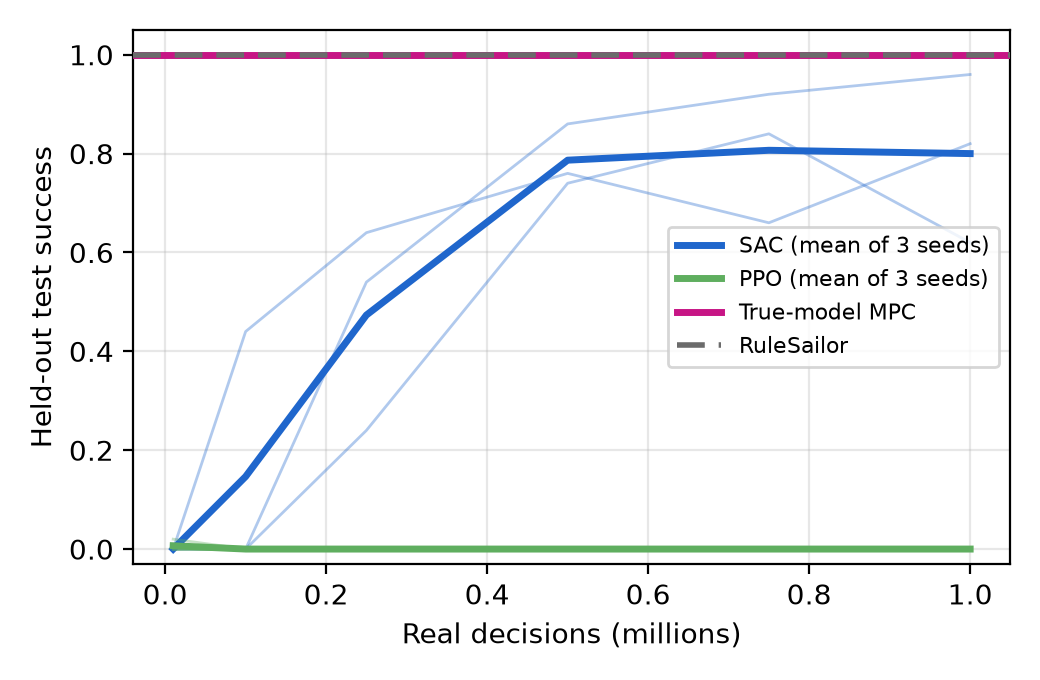
\includegraphics[width=\textwidth]{r_learning.png}
    \end{column}
    \begin{column}{0.42\textwidth}
      \small
      \begin{tabular}{@{}lrr@{}}
        \toprule
        Finishes             & Test           & Shift \\
        \midrule
        \PPO                 & \rPPOtest      & \rPPOshift \\
        \SAC                 & \rSACtest      & \rSACshift \\
        \MPC{} (true model)  & \rMPCtest      & \rMPCshift \\
        \Rule                & \rRULEtest     & \rRULEshift \\
        \bottomrule
      \end{tabular}\\[0.6em]
      {\scriptsize Learners: 3 training seeds, validation-selected checkpoints.
       MPC: 3 search seeds. RuleSailor: hand-written reference.}\\[0.8em]
      \SAC{} learns the reach in about 0.5M decisions; \PPO{} never finds the gate.
    \end{column}
  \end{columns}
\end{frame}

% ---------------------------------------------------------------- 2:25
\begin{frame}{Results upwind (U, preliminary): the tack is the bottleneck}
  \begin{columns}[c]
    \begin{column}{0.55\textwidth}
      \centering
      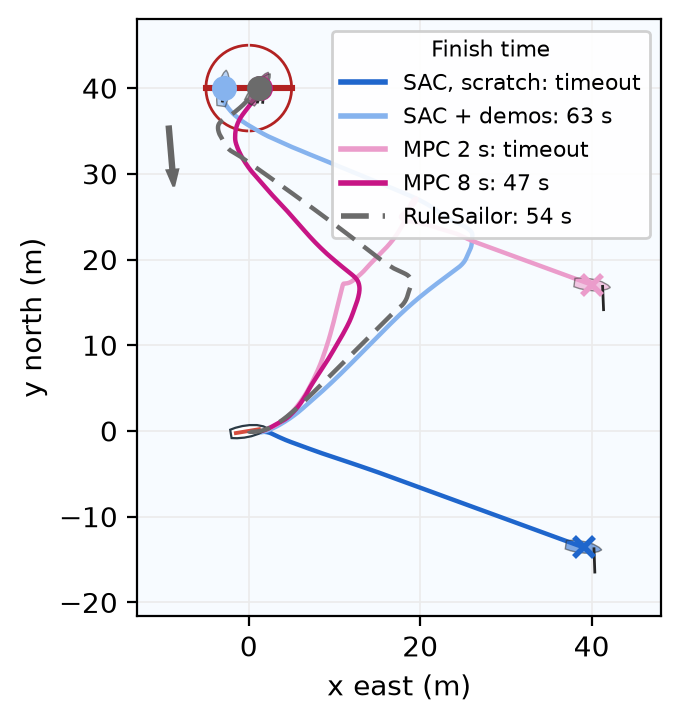
\includegraphics[height=0.72\textheight]{u_tracks.png}\\
      {\scriptsize First validation condition (5.1\,m/s from N), one seed each}
    \end{column}
    \begin{column}{0.43\textwidth}
      \footnotesize
      \begin{tabular}{@{}lr@{}}
        \toprule
        Finishes (test, 3 seeds $\times$ 50)  & \\
        \midrule
        \textcolor{colPPO}{PPO, PPO $+$ BC, BC only} (each) & \uPPOtest \\
        \SAC                                  & \uSACtest \\
        \SAC{} $+$ demonstrations             & \uSACDtest \\
        \Rule{} (1 run)                       & \uRULEtest \\
        \midrule
        \MPC{} 2\,s horizon (validation)      & \uMPCvalShort \\
        \MPC{} 8\,s horizon (validation)      & \uMPCvalLong \\
        \MPC{} 8\,s horizon (test)            & \uMPCtest \\
        \bottomrule
      \end{tabular}\\[0.3em]
      {\scriptsize\uMPCpartial}\\[0.6em]
      \alert{Planning is horizon-bound:} 8\,s always tacks but needs \uMPCpLong\,ms per decision
      (offline). \alert{Learners never find the tack} in 4M decisions.
    \end{column}
  \end{columns}
\end{frame}

% ---------------------------------------------------------------- 2:50
\begin{frame}{Takeaways and next steps}
  \begin{itemize}
    \item \alert{Known model + long enough horizon} (\MPC): reliable, but not real-time upwind
    \item \alert{Reusing experience} (\SAC) beats fresh batches (\PPO) on the reach
    \item Upwind is an \alert{exploration} problem: from scratch no learner tacks;
          expert data helps only a little
  \end{itemize}
  \vspace{1em}
  \begin{block}{Next (final presentation, Dec 3)}
    Finish the upwind held-out evaluation; diagnose tacks, irons and mark misses from exact
    replays; claim-to-evidence index for every number.
  \end{block}
\end{frame}

\end{document}
